\documentclass{article}
\usepackage{pgfplots}
\pgfplotsset{compat=1.17}
\begin{document}
\section{Pictures}
Mapping a dataflow graph onto a coarse-grained array asks the compiler to place every operation and route every value in space and time, and the search grows with the fabric.

\begin{figure}[h]\centering
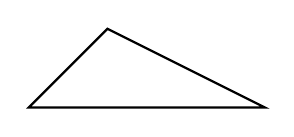
\begin{tikzpicture}\draw[thick] (0,0) -- (1,1) -- (3,0) -- cycle;\end{tikzpicture}
\caption{A triangle.}\label{fig:t}\end{figure}
Mapping a dataflow graph onto a coarse-grained array asks the compiler to place every operation and route every value in space and time, and the search grows with the fabric.

\begin{figure}[h]\centering
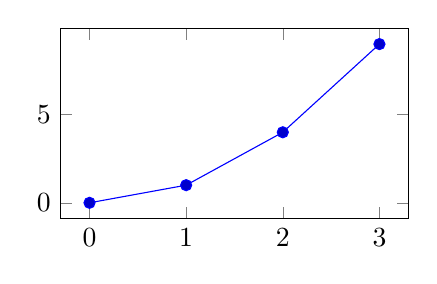
\begin{tikzpicture}\begin{axis}[width=6cm,height=4cm]\addplot coordinates {(0,0) (1,1) (2,4) (3,9)};\end{axis}\end{tikzpicture}
\caption{A plot.}\label{fig:plot}\end{figure}
Mapping a dataflow graph onto a coarse-grained array asks the compiler to place every operation and route every value in space and time, and the search grows with the fabric.
\end{document}
